\documentclass{article}

\usepackage[utf8]{inputenc}
\usepackage[T1]{fontenc}
%\usepackage[latin1]{inputenc}
%\usepackage[utf8]{fontenc}
\usepackage{amsmath}
\usepackage{amsfonts}
\usepackage{amssymb}
\usepackage{amsthm}
\usepackage{graphicx}
\usepackage{pifont}

\newtheorem*{definition}{Definition}
\newtheorem*{theorem}{Theorem}
\newtheorem*{example}{Example}
\setlength{\parskip}{2pt}
\newcommand{\argmax}{\operatornamewithlimits{argmax}}

\author{Emmanuel Rachelson}
\title{Support Vector Machines and kernels}
\date{}

\begin{document}

\maketitle



\noindent Consider a training set $\mathcal{D}= \left\{(x_i,y_i)\right\}_{i\in [1,N]}$ where $x_i\in\mathbb{R}^n$ and $y_i\in\left\{-1;1\right\}$. Support Vector Machines for classification find the best possible separating hyperplane in $\mathbb{R}^n$ in order to scatter $\mathcal{D}$, according to a criterion that maximizes a compromise between the correct classification of all data points and the margin obtained. For this purpose, it requires solving a quadratic programming problem. In the regression case ($y_i \in\mathbb{R}$), Support Vector Regression fits a hyperplane to the data by optimizing a compromise between flatness and a loss function that quantifies how far data points are from the hyperplane. Extension to non-linear separation or regression surfaces is made possible by the kernel trick.

This synthesis is essentially built upon the two following articles:\\
\textbf{A tutorial on Support Vector Machines for Pattern Recognition.} C. J. C. Burges, \textit{Data Mining and Knowledge Discovery}, \textbf{2}, 111--167, (1998).\\
\textbf{A tutorial on Support Vector Regression.} A. J. Smola and B. Sch\"olkopf, \textit{Journal of Statistics and Computing}, \textbf{14}(3), 199--222, (2004).

\section*{Linear classification on linearly separable data}

\textbf{Maximizing the margin.} 
Consider the problem of separating white and black dots in Figure \ref{fig:lin-lin} using a hyperplane (a line, in $\mathbb{R}^2$).
\begin{figure}
\begin{center}
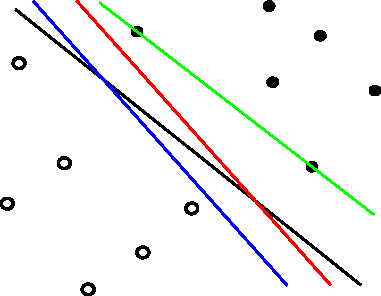
\includegraphics[width=6cm]{../img/lin_sep2.pdf}
\end{center}
\caption{Linear separating hyperplanes}
\label{fig:lin-lin}
\end{figure}

In this section we assume the points are indeed separable linearly, \emph{ie.} such a hyperplane does exist. Let $w^Tx+b = 0$ be the equation of this hyperplane with normal unit vector $w \in \mathbb{R}^n$ ($\|w\|=1$) and intercept $\frac{b}{\|w\|}=b$. Any valid separating hyperplane verifies:
\begin{align*}
w^Tx_i + b \geq 0 \text{ for } y_i=+1\\
w^Tx_i + b \leq 0 \text{ for } y_i=-1
\end{align*}
Note that $y_i\left( w^Tx_i + b \right)$ is the signed distance from any point $x_i$ to the hyperplane. If this quantity is negative (resp. positive) the point is on the ``wrong'' (resp. ``right'') side of the hyperplane. The larger its absolute value, the further the point is from the hyperplane. Then the above constraints can be summarized as:
\begin{align*}
\forall i \in [1;N], \ y_i\left( w^Tx_i + b \right) \geq 0
\end{align*}

From a geometric point of view, the best separating hyperplane is the one that stands as far as possible from any point while still respecting the previous constraint. In other words, it is the one that maximizes the distance to the closest point. Let $M_+$ be the distance to the closest point with $y_i=+1$ and $M_-$ the distance to the closest point with $y_i=-1$. Then one defines the \emph{margin} of the separating hyperplane as the sum $M=M_+ + M_-$.

The Support Vector Machine algorithm looks for the separating hyperplane that maximizes the margin. This can be expressed as:
\begin{gather*}
\max_{w,b} M\\
\text{such that } \forall i \in [1;N], \ y_i\left( w^Tx_i + b \right) \geq M \text{ and } \|w\| = 1
\end{gather*}

\textbf{A quadratic optimization problem.} 
This formulation can be simplified by introducing $w'= \frac{1}{M} w$ and $b'=\frac{1}{M} b$. By dividing the constraints by $M$, one obtains $y_i\left( w'^Tx_i + b' \right) \geq 1$. Since $\|w\|=1$, $M=\frac{1}{\|w'\|}$ and maximizing the margin is equivalent to minimizing $\|w'\|$ or $\|w'\|^2$. Thus one can eliminate $M$ from the above optimization problem, which becomes (we drop the $w'$ notation):
\begin{gather*}
\min_{w,b} \frac{1}{2} \|w\|^2 \\
\text{such that } \forall i \in [1;N], \ y_i\left( w^Tx_i + b \right) \geq 1
\end{gather*}

The above problem is the canonical form of the linear SVM formulation in the separable case. It is a quadratic programming problem since the objective function is quadratic in the variables $w$ and $b$ and since the $N$ constraints are linear in $w$ and $b$.

We introduce the Lagrange multipliers $\alpha_i$ for each constraint and write the Lagrangian of this problem:
\begin{equation*}
L(w,b,\alpha) = \frac{1}{2} \|w\|^2 + \sum_{i=1}^N \alpha_i\left(1-y_i\left( w^Tx_i + b \right)\right)
\end{equation*}

All the constraints are linear, thus qualified, and one can use the Karush-Kuhn-Tucker (KKT) theorem to derive necessary and sufficient conditions to find optimal $w$ and $b$ values. Since, additionaly, the objective function and constraints are convex, one can use the duality theorem that states that the solution to the optimization problem is also the solution to:
\begin{equation*}
\max_{\alpha \geq 0} \min_{w,b} L(w,b,\alpha)
\end{equation*}

In order to solve this problem we use KKT's first order necessary condition. Any candidate solution must satisfy:
\begin{align*}
&\frac{\partial L}{\partial w} = w - \sum_{i=1}^N \alpha_i y_i x_i = 0\\
&\frac{\partial L}{\partial b} = \sum_{i=1}^N \alpha_i y_i = 0\\
&\forall i\in [1;N], \ \alpha_i\left(1-y_i\left( w^Tx_i + b \right)\right) = 0\\
&\forall i\in [1;N], \ \alpha_i \geq 0
\end{align*}

The first two equations above correspond to the minimization term in the application of the duality theorem. From them we get:
\begin{gather*}
w= \sum_{i=1}^N \alpha_i y_i x_i\\
\sum_{i=1}^N \alpha_i y_i = 0
\end{gather*}

We replace $w$ by its expression as a function of $\alpha$ in the primal function:
\begin{align*}
L(w,b,\alpha) &= \frac{1}{2} \left\|\sum_{i=1}^N \alpha_i y_i x_i\right\|^2 + \sum_{i=1}^N \alpha_i\left(1-y_i\left( \left(\sum_{j=1}^N \alpha_j y_j x_j\right)^Tx_i + b \right)\right)\\
&= \frac{1}{2} \sum_{i=1}^N \sum_{j=1}^N  \alpha_i \alpha_j y_i y_j x_i^T x_j + \sum_{i=1}^N \alpha_i - \sum_{i=1}^N \sum_{j=1}^N  \alpha_i \alpha_j y_i y_j x_i^T x_j - \left(\sum_{i=1}^N \alpha_i y_i\right) b\\
&= \sum_{i=1}^N \alpha_i - \frac{1}{2} \sum_{i=1}^N \sum_{j=1}^N  \alpha_i \alpha_j y_i y_j x_i^T x_j
\end{align*}

This forms the dual function $L_D(\alpha)$ which needs to be minimized over positive values of $\alpha_i$ to find the optimum $w$ and $b$. The dual problem is thus:
\begin{gather*}
\max_{\alpha \geq 0} \sum_{i=1}^N \alpha_i - \frac{1}{2} \sum_{i=1}^N \sum_{j=1}^N  \alpha_i \alpha_j y_i y_j x_i^T x_j\\
\text{such that }\sum_{i=1}^N \alpha_i y_i = 0
\end{gather*}
This dual problem can be solved through a variety of optimization algorithms, the most commonly used being Sequential Minimal Optimization (SMO), implemented in most modern SVM libraries and introduced in:\\
\textbf{Fast training of support vector machines using sequential minimal optimization.} J. Platt, \textit{Advances in Kernel Methods}, 185–-208, (1999).

\textbf{Support vectors.} Overall, the general form of $w$ is given by:
\begin{equation*}
w= \sum_{i=1}^N \alpha_i y_i x_i
\end{equation*}
That means $w$ is a linear combination of the $x_i$, with coefficients $\alpha_i y_i$. Consider the $\alpha_i\left(1-y_i\left( w^Tx_i + b \right)\right) = 0$  condition. It states that if $y_i\left( w^Tx_i + b \right) > 1$, that is if $x_i$ lies strictly \emph{outside} the margin, then the corresponding multiplier $\alpha_i$ is necessarily zero, and $x_i$ does not participate in the linear combination defining $w$.

In other words, $w$ is defined by the $x_i$ for which $\alpha_i > 0$, which implies in turn that for these $x_i$, $y_i\left( w^Tx_i + b \right) = 1$: these points lie on the margin boundary. Such points are called \emph{Support Vectors} as illustrated on Figure \ref{fig:lin-lin2}.

\begin{figure}
\begin{center}
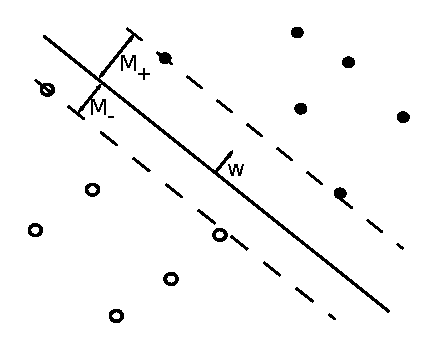
\includegraphics[width=6cm]{../img/lin_sep3.pdf}
\end{center}
\caption{Support Vectors}
\label{fig:lin-lin2}
\end{figure}

Interestingly, all points which are not support vectors can be removed from the problem and the solution $w$ will remain the same. The support vectors are the points lying on the margin's boundary, hence one can expect their number in practice to be much smaller than $N$. For this reason, SVM are called \emph{sparse} linear classifiers: the majority of coefficients of $x_i$ in the $w$ linear combination are zero. Thus, storing an SVM boils down to storing the support vectors and their coefficients.

Finally, only $b$ remains to be determined. This is feasible via any of the $y_i\left( w^Tx_i + b \right) = 1$ constraints (constraints for which $\alpha_i\neq 0$). However it is numerically safer to take the average of the values of $b$ resulting from these constraints. Let $SV$ be the set of support vector indices, then:

\begin{equation*}
b = \frac{1}{\text{card}(SV)} \sum_{i \in SV} \left[ \frac{1}{y_i} - w^T x_i \right] = \frac{1}{\text{card}(SV)} \sum_{i \in SV} \left[ \frac{1}{y_i} - \sum_{j=1}^N \alpha_j y_j x_j^T x_i \right]
\end{equation*}

\textbf{Classifying new data.} In order to predict the class of a new data point $x$, one needs to take the sign of $w^Tx+b$. So the predicted class $y$ is:
\begin{equation*}
y = \text{sign}\left( \sum_{i=1}^N \alpha_i y_i x_i^T x + b \right)
\end{equation*}

Note that this computation boils down to calculating the dot product of $x$ with all support vectors and computing the weighted sum of the results. This remark will come in handy further in this document.

\section*{Linear classification on non linearly separable data}

\textbf{Slack variables.} The next step consists in generalizing the previous approach in order to build separating hyperplanes for non-linearly separable data as illustrated in Figure \ref{fig:nlin-lin}. Obviously, in this case, the $y_i\left( w^Tx_i + b \right) \geq 1$ constraints yield an empty set of solutions (if the data is not linearly separable, there exists no hyperplane shattering the points). Consequently, one must introduce some slack in the formulation, by allowing some points $x_i$ to be \emph{inside} the margin boundaries or even \emph{misclassified}. For this purpose, we introduce the \emph{slack variables} $\xi_i \geq 0$ such that:
\begin{equation*}
y_i\left( w^Tx_i + b \right) \geq M(1-\xi_i)
\end{equation*}
\begin{figure}
\begin{center}
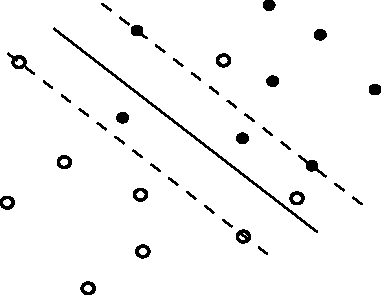
\includegraphics[width=6cm]{../img/non_lin_sep1.pdf}
\end{center}
\caption{Linear classification on non linearly separable data}
\label{fig:nlin-lin}
\end{figure}
Thus, $\xi_i=0$ shall stand for points outside or touching the margin boundary, $\xi_i \in[0;1]$ will describe points correctly classified but inside the margin, and $\xi_i>1$ will denote misclassified points. So the optimal separating hyperplane needs to make a compromise between maximizing the margin and minimizing $\sum_{i=1}^N \xi_i$. By using the same trick as earlier in order to eliminate $M$, one obtains the general formulation: 
\begin{gather*}
\min_{w,b} \frac{1}{2} \|w\|^2 + C \sum_{i=1}^N \xi_i\\
\text{such that } \forall i \in [1;N], \ y_i\left( w^Tx_i + b \right) \geq 1-\xi_i\\
\text{and } \forall i \in [1;N], \ \xi_i \geq 0
\end{gather*}

This is still a quadratic programming problem. We introduce the Lagrange multipliers $\alpha_i$ for the $y_i\left( w^Tx_i + b \right) \geq 1-\xi_i$ constraint, and $\mu_i$ for the $\xi_i\geq 0$ constraint. The problem's Lagrangian is now:
\begin{equation*}
L(w,b,\xi,\alpha, \mu) = \frac{1}{2} \|w\|^2 + C \sum_{i=1}^N \xi_i + \sum_{i=1}^N \alpha_i\left(1-\xi_i-y_i\left( w^Tx_i + b \right)\right) - \sum_{i=1}^N \mu_i \xi_i
\end{equation*}

KKT's first order necessary condition writes:
\begin{align*}
&\frac{\partial L}{\partial w} = w - \sum_{i=1}^N \alpha_i y_i x_i = 0\\
&\frac{\partial L}{\partial b} = \sum_{i=1}^N \alpha_i y_i = 0\\
&\frac{\partial L}{\partial \xi_i} = -\alpha_i + C - \mu_i = 0\\
&\forall i\in [1;N], \ \alpha_i\left(1-\xi_i-y_i\left( w^Tx_i + b \right)\right) = 0\\
&\forall i\in [1;N], \ \alpha_i \geq 0\\
&\forall i\in [1;N], \ \mu_i\xi_i = 0\\
&\forall i\in [1;N], \ \mu_i \geq 0
\end{align*}
By factoring the $\xi_i$ variables together in the Lagrangian we obtain:
\begin{equation*}
L(w,b,\xi,\alpha, \mu) = \frac{1}{2} \|w\|^2 + \sum_{i=1}^N (C-\alpha_i-\mu_i)\xi_i + \sum_{i=1}^N \alpha_i\left(1-y_i\left( w^Tx_i + b \right)\right)
\end{equation*}

As previously, we use the first three equations to derive the dual function which is finally the same as in the previous problem:
\begin{equation*}
L_D(\alpha, \mu) = \sum_{i=1}^N \alpha_i - \frac{1}{2} \sum_{i=1}^N \sum_{j=1}^N  \alpha_i \alpha_j y_i y_j x_i^T x_j
\end{equation*}

The dual problem is thus:
\begin{gather*}
\max_{\alpha, \mu\geq 0} \sum_{i=1}^N \alpha_i - \frac{1}{2} \sum_{i=1}^N \sum_{j=1}^N  \alpha_i \alpha_j y_i y_j x_i^T x_j\\
\text{such that } \sum_{i=1}^N \alpha_i y_i = 0\\
\text{and }\forall i\in [1;N], \ -\alpha_i + C - \mu_i = 0
\end{gather*}

One can finally eliminate the $\mu_i$ variables by remarking that $-\alpha_i + C - \mu_i = 0$ and $\mu_i\geq 0$ boils down to $\alpha_i\leq C$. The final form of the dual problem is thus:
\begin{gather*}
\max_{0\leq\alpha\leq C} \sum_{i=1}^N \alpha_i - \frac{1}{2} \sum_{i=1}^N \sum_{j=1}^N  \alpha_i \alpha_j y_i y_j x_i^T x_j\\
\text{such that } \sum_{i=1}^N \alpha_i y_i = 0
\end{gather*}

Consequently, finding the optimal $\alpha_i$ is the same process as in the previous case.

\textbf{Support vectors.} Again, the general expression of $w$ is:
\begin{equation*}
w = \sum_{i=1}^N \alpha_i y_i x_i
\end{equation*}
So $w$ is a linear combination of the $x_i$.

If $y_i\left( w^Tx_i + b \right) > 0$, that is if $x_i$ is well classified and not on the margin's border, then necessarily $\alpha_i = 0$. As previously, these points are not support vectors and do not participate in the linear combination defining $w$.

On the other hand, for $y_i\left( w^Tx_i + b \right) = 0$ one has $\alpha_i \geq 0$ and needs to distinguish two cases. If $\xi_i>0$, that is if $x_i$ is a support vector inside the margin boundaries (possibly misclassified), then necessarily $\mu_i=0$ and then $\alpha_i = C$. If, however, $\xi_i=0$, that is if $x_i$ is a support vector defining the margin's boundary, then $\mu_i \geq 0$ and $\alpha_i \in ]0;C]$. To summarize, the training points fall into three categories as illustrated by Figure \ref{fig:nlin-lin2}:
\begin{itemize}
\item Non support vector, $\alpha_i = 0$.
\item Support vector defining the margin's boundary, $\alpha_i \in ]0:C]$
\item Support vector inside the margin's boundary, $\alpha_i=C$
\end{itemize}
\begin{figure}
\begin{center}
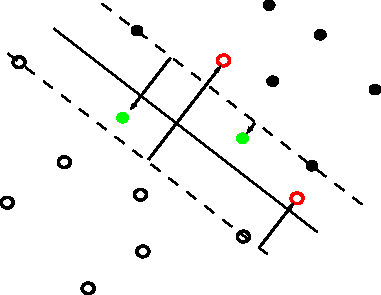
\includegraphics[width=6cm]{../img/non_lin_sep3.pdf}
\end{center}
\caption{Support vectors in the non linearly separable case}
\label{fig:nlin-lin2}
\end{figure}

Again, non support vectors could be removed from the training set and the optimization result would still be the same. Finally, determining $b$, as previously, can be done by using the constraint $\alpha_i\left(1-\xi_i-y_i\left( w^Tx_i + b \right)\right)=0$ on points for which $\alpha_i>0$ (support vectors) and $\xi_i=0$. These points can be found for example by taking the $\alpha_i$ that are strictly between 0 and $C$ (because if $\alpha_i<C$, then $\mu_i>0$ and $\xi_i=0$). As previously, it is numerically preferable to average the value of $b$ over all such points. Let $I$ be the set of indices of the data points for which $0<\alpha_i<C$, then $b$ is:
\begin{equation*}
b = \frac{1}{\text{card}(I)} \sum_{i \in I} \left[ \frac{1}{y_i} - \sum_{j=1}^N \alpha_j y_j x_j^T x_i \right]
\end{equation*}

\textbf{Classifying new data.} Exactly as in the previous case, in order to predict the class of a new data point $x$, one needs to take the sign of $w^Tx+b$. So the predicted class $y$ is:
\begin{equation*}
y = \text{sign}\left( \sum_{i=1}^N \alpha_i y_i x_i^T x + b \right)
\end{equation*}

\textbf{Trade-off factor $C$.} Choosing a value for $C$ has much impact on the optimization result. If $C$ is large, then the emphasis will be put on classifying correctly as many points as possible, with the risk of overfitting the data. On the contrary, a small value of $C$ will lead to a margin as large as possible, tolerating many misclassifications at the risk of missing some fine specificities in the data. The optimal value for $C$ is usually found via cross-validation on the training set.

\section*{The kernel trick and its application to SVM}

So far, we have presented SVMs as a purely linear classifier and developped the theory that allows to construct optimal separating hyperplanes. Implicitly, we made the assumption that although the data might not be linearly separable, the general structure behind the data could be captured by a linear classifier (the non separability being due, for example, to measurement noise). This assumption does not hold in many real world situations and it would be desirable to extend the elegant framework of SVMs to non-linear classifiers. Consider for instance the data represented in Figure \ref{fig:datamix}. Although it is possible to construct the optimal linear SVM for this data for any value of the trade-off parameter $C$, no hyperplane obtained this way will be satisfying simply because intrinsically, the data was not generated by a linear classification function. Fortunately, the \emph{kernel trick} and the theory of Reproducing Kernel Hilbert Spaces (RKHS) allow us to straightforwardly extend linear classifiers to the non-linear case. We will only skim the surface of this theory of kernel function in this section, prefering a gentle introduction to its foundations and practice.

\begin{figure}
\begin{center}
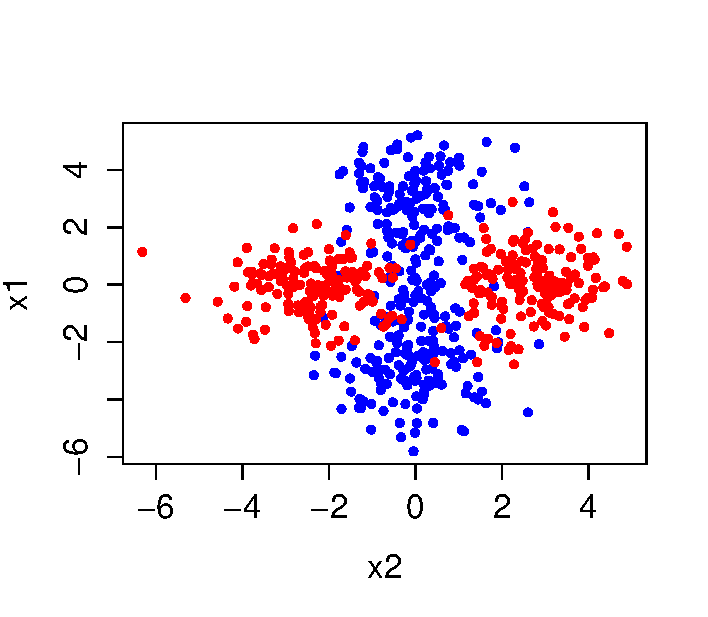
\includegraphics[width=8cm]{../img/datamix.pdf}
\end{center}
\caption{Non linearly separable data}
\label{fig:datamix}
\end{figure}

\textbf{Hilbert spaces.} We start with a remark. Suppose one provides a mapping $h$ from $\mathbb{R}^n$ to a Hilbert space $\mathcal{H}$ of dimension $p\gg n$. Recall at the occasion that a Hilbert space is a generalization of a Euclidean space, that is a vector space (possibly of infinite dimension) equipped with an inner product and complete with respect to this inner product. To make the reading slightly easier and fix ideas, it is possible to replace ``Hilbert space'' by ``Euclidean space'' in what follows.
\begin{equation*}
h:\left\{\begin{array}{ccc}\mathbb{R}^n &\rightarrow & \mathcal{H}\\x &\mapsto& h(x)\end{array}\right.
\end{equation*}
Now take the image $x'_i = h(x_i)$ of each point $x_i$ from the training set and build the optimal separating hyperplane in $\mathcal{H}$ as shown in the previous section. This hyperplane has normal vector $w'=\sum_{i=1}^N \alpha_i y_i h(x_i)$  and intercept $b'$, and hence, classifying a new point $x\in \mathbb{R}^n$ can be done by taking its image $h(x)$ and checking the sign of $w'^T h(x) + b'$:
\begin{align*}
y &= \text{sign}\left( w'^T h(x) + b' \right)\\
&= \text{sign}\left( \sum_{i=1}^N \alpha_i y_i h(x_i)^T h(x) + b' \right)
\end{align*}

Suppose now that one knows a function $K(x_1,x_2)$ which computes precisely the inner product $h(x_1)^T h(x_2)$. Then the prediction function becomes:
\begin{equation*}
y = \text{sign}\left( \sum_{i=1}^N \alpha_i y_i K(x_i,x) + b' \right)
\end{equation*}

This $K$ function is called a \emph{kernel function}. Intuitively, it  projects its two arguments in a different Hilbert space and computes the inner product of the images.

The key interest of such an operation is that although the data might not be linearly separable in $\mathbb{R}^n$ (as the data of Figure \ref{fig:datamix} for instance) there might exist another space $\mathcal{H}$ (usually of higher dimension) in which separating linearly the images of the $x_i$ points makes more sense. If $K(\cdot,\cdot)$ is  indeed an inner product in this space, then one does not even need to know the mapping $h$ to evaluate the SVM.

Now this works if the SVM has already been computed in $\mathcal{H}$ and we only need to do evaluation. Let us take a second look at the determination of the SVM's key parameters $\alpha_i$ and $b'$. The optimal values of the Lagrange multipliers $\alpha_i$ are found by solving the dual problem:
\begin{gather*}
\max_{0\leq\alpha\leq C} \sum_{i=1}^N \alpha_i - \frac{1}{2} \sum_{i=1}^N \sum_{j=1}^N  \alpha_i \alpha_j y_i y_j h(x_i)^T h(x_j)\\
\text{such that } \sum_{i=1}^N \alpha_i y_i = 0
\end{gather*}
The dual function features only inner products of elements of $\mathcal{H}$ and never manipulates these elements alone. Thus, we can replace $h(x_i)^T h(x_j)$ by $K(x_i,x_j)$ and the dual problem becomes: 
\begin{gather*}
\max_{0\leq\alpha\leq C} \sum_{i=1}^N \alpha_i - \frac{1}{2} \sum_{i=1}^N \sum_{j=1}^N  \alpha_i \alpha_j y_i y_j K(x_i,x_j)\\
\text{such that } \sum_{i=1}^N \alpha_i y_i = 0
\end{gather*}
Solving this problem and finding the optimal $\alpha_i$ never requires actually computing the image $h(x_i)$ of any point $x_i$.

Similarly, determining $b'$ only uses inner products of elements of $\mathcal{H}$ and never these elements themselves. Let $I$ be the set of indices of the data points for which $0<\alpha_i<C$, then $b'$ is:
\begin{align*}
b' &= \frac{1}{\text{card}(I)} \sum_{i \in I} \left[ \frac{1}{y_i} - \sum_{j=1}^N \alpha_j y_j h(x_j)^T h(x_i) \right]\\
&= \frac{1}{\text{card}(I)} \sum_{i \in I} \left[ \frac{1}{y_i} - \sum_{j=1}^N \alpha_j y_j K(x_j, x_i) \right]
\end{align*}

Consequently, in order to compute the optimal separating hyperplane in $\mathcal{H}$ and to use it to classify points of $\mathbb{R}^n$, one never needs to explicitly compute any mapping from $\mathbb{R}^n$ to $\mathcal{H}$, but rather needs to know a \emph{kernel function} $K(\cdot,\cdot)$ which represents \emph{any} inner product in $\mathcal{H}$. Actually, it is not even necessary to have an explicit knowledge of what $\mathcal{H}$ is: as long as one can guarantee that $K(\cdot,\cdot)$ is an inner product in some Hilbert space, then it is possible to compute an optimal separating hyperplane in this Hilbert space and use it to classify elements of $\mathbb{R}^n$ without ever needing to compute their images in this Hilbert space.

This fascinating property is called the \emph{kernel trick}.

\textbf{Positive definite kernels.} So the next question is: how does one know a function $K(\cdot,\cdot)$ has the properties of an inner product over a Hilbert space? In other words, how does one know that there exists a Hilbert space $\mathcal{H}$ and a mapping $h$ into that space such that $K(\cdot,\cdot)$ is an inner product on $\mathcal{H}$? The answer is provided by Mercer's condition:

Given a function $K:X\times X \rightarrow \mathbb{R}$, there exists a Hilbert space $\mathcal{H}$ and a mapping $h:X\rightarrow\mathcal{H}$ such that $K(x_1,x_2)$ is the inner product of $h(x_1)$ and $h(x_2)$ if and only if for any function $g$ with finite $L_2$ norm:
\begin{equation*}
\forall g(x) / \int g(x)^2dx <\infty, \iint K(x,y)g(x)g(y)dxdy \geq 0
\end{equation*}

\textbf{Examples of kernels.} Obviously, if one can explicitly construct the mapping $h$, then it is easy to derive the corresponding kernel $K$. Most often however, kernels are functions for which Mercer's condition has been verified.

For example:
\begin{itemize}
\item The polynomial kernel $K(x,y)=\left(1+\langle x, y\rangle\right)^d$
\item The radial basis function (a.k.a. Gaussian) kernel $K(x,y) = e^{-\gamma \|x-y\|^2}$ (very often used in $\mathbb{R}^n$)
\item The sigmoid kernel $K(x,y) = \tanh\left(\kappa_1 \langle x, y\rangle + \kappa_2\right)$
\end{itemize}

Note that the dimension of the corresponding Hilbert spaces is sometimes known. For example for the polynomial kernel, it is finite and equal to $\frac{(n+d-1)!}{d!(n-1)!}$. For the radial basis function kernel it is infinite. Note also that the sigmoid kernel does not satisfy Mercer's condition for all values of $\kappa_1$ and $\kappa_2$.

In this presentation, we have supposed all along for ease of presentation that the data $x_i$ lived in $\mathbb{R}^n$. It is possible to straightforwardly generalize this assumption to any space $X$ as long as it is possible to construct a positive definite kernel on $X$. Imagine for example that $X$ is the space of all possible chromosomes, then $K$ needs to be defined over $X\times X$ in order to build an SVM that does genetic classification.

To summarize this Section, the kernel trick allows one to construct non-linear SVM, which are optimal separating hyperplanes in the Hilbert space corresponding to the kernel used.

Figure \ref{fig:datamix_svm} shows an example of an SVM trained with a radial basis function kernel on the data of Figure \ref{fig:datamix} (support vectors appear in black).

\begin{figure}
\begin{center}
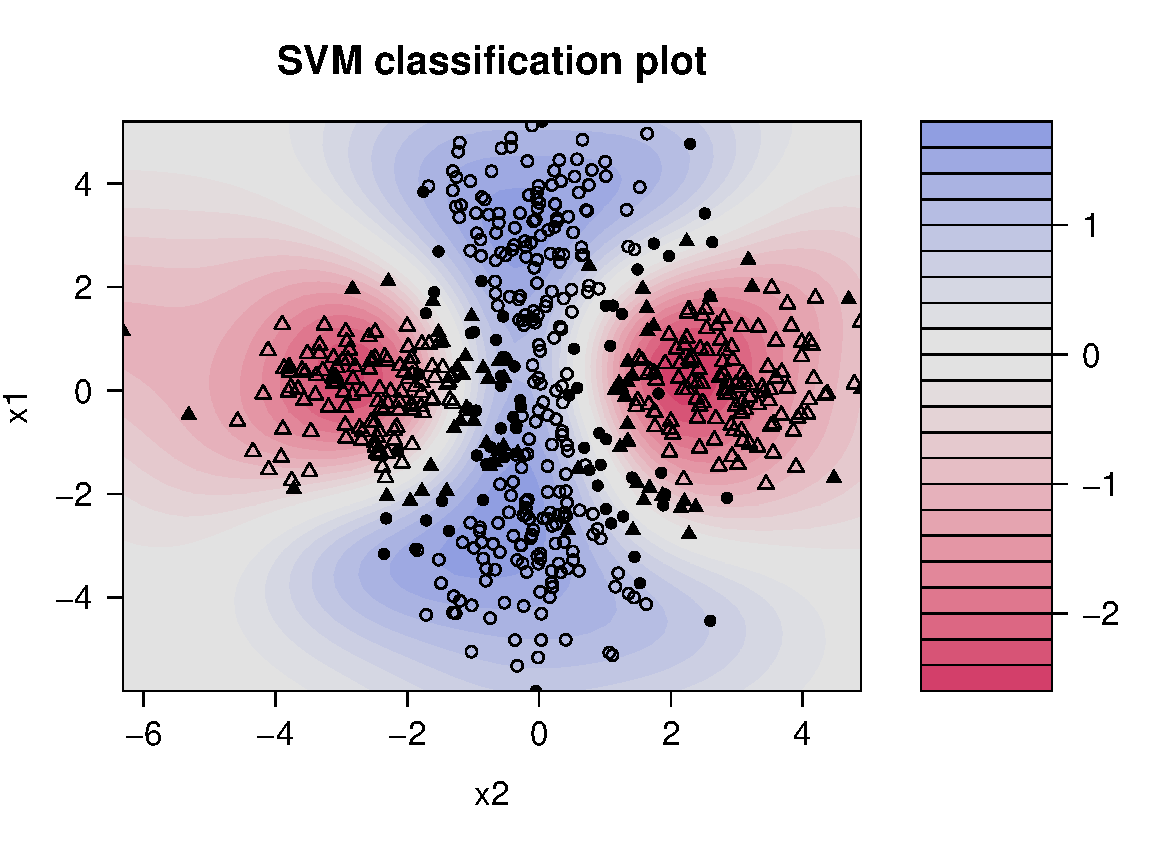
\includegraphics[width=10cm]{../img/datamix_svm.pdf}
\end{center}
\caption{Non-linear SVM with RBF kernel}
\label{fig:datamix_svm}
\end{figure}

\section*{Support Vector Regression}

In this section, we shall start with the problem of linear regression in SVMs and then generalize (via the kernel trick again) to non-linear functions.

The understanding of regression problems differs slightly from the classification case. In a regression problem, one needs to guide a regression function through the regression points, contrarily to the classification case where one wanted to have the separating surface as far as possible from the points in order to maximize the margin. So deriving the same type of optimization problem as in the classification case, namely minimizing $\|w\|^2$ under constraints that penalize the gap between $w^Tx_i+b$ and $y_i$, cannot be interpreted in terms of margin.

Minimizing $\|w\|^2$ however still makes sense for other reasons. Such a minimization corresponds to looking for the most ``horizontal'' hyperplane possible or the flatest hyperplane possible (here, ``flat'' is understood in the sense of ``as orthogonal as possible to the $y$ axis''). This means one looks for $w_i$ values as small as possible. Such a goal is known as \emph{ridge regression} or more generally \emph{Tikhonov regression} and in the Machine Learning litterature it corresponds to an operation called \emph{regularization}. Regularization imposes a penalty on the value of the coefficients $w_i$ in the optimization problem that best describes the fitting hyperplane. The justification and the intuition behind regularization can be understood as follows:
\begin{itemize}
\item Suppose the training data is noisy and some mesures $y_i$ are over-evaluated compared to their true value. Then, forcing the fitting hyperplane to have as small values $w_i$ as possible makes its training more robust to noise. Prediction is then less sensitive to training noise (because the values of $w_i$ are small).
\item Consider also that one of the features describing the data is completely irrelevant. Then one would wish the prediction to depend as little as possible on this feature and hence to have a corresponding $w_i$ as small as possible. In other words, minimizing $\|w\|$ is a way of performing feature selection: only the ones that have strong explanatory power have noticeable values while all other ones are pulled down to zero. One can view this principle as an application of \emph{Occam's razor}. It is a component-wise penalization of $w$.
\item In the context of SVMs, since $w$ is a linear combination of the $x_i$, penalizing $\|w\|$ is a way of pulling most $\alpha_i$ down to zero and thus enforcing parsimony (sample sparsity).
\end{itemize}
In principle, for component-wise and sample sparsity, the penalization of $w$ should be done by taking the L0 norm (the number of non-zero elements), however this one is non-differentiable and it is easier to use the L2 norm. Some cases (such as LASSO regression for instance) take advantage of L1 regularization. More on this crucial topic:\\
\textbf{Feature selection, L1 vs. L2 regularization, and rotational invariance.} Andrew Y. Ng, \textit{International Conference on Machine Learning}, 2004.\\
\textbf{Regression shrinkage and selection via the LASSO.} Robert Tibshirani, \textit{Journal of the Royal Statistical Society}, Series B, \textbf{58}(1):267--288, 1996.

Consequently, the objective function of the Support Vector Regression (SVR) problem is a compromise between fitting the hyperplane to the data and penalizing $\|w\|$. The fitting part makes use of a \emph{loss function} $V(\cdot)$ that quantifies how much a loss $y_i-w^T x_i + b$ should weight in the objective function.
\begin{equation*}
\min\limits_{w,b} \frac{1}{2} \|w\|^2 + C \sum\limits_{i=1}^N V(y_i-w^T x_i + b))
\end{equation*}

The most common loss functions used are:\\
\begin{tabular}{ll}
$\epsilon$-insensitive & $V(z) = \left\{\begin{array}{l} 0\text{ if }|z|\leq\epsilon\\ |z|-\epsilon\text{ otherwise}\end{array}\right.$\\
Laplacian & $V(z) = |z|$\\
Gaussian & $V(z) = \frac{1}{2}z^2$\\
Huber's robust loss & $V(z) = \left\{\begin{array}{l}\frac{1}{2\sigma}z^2\text{ if }|z|\leq\sigma \\ |z|-\frac{\sigma}{2}\text{ otherwise}\end{array}\right.$\\
\end{tabular}

We shall focus on the $\epsilon$-insensitive loss function (also called \emph{soft margin loss}) as it is the most used. As illustrated on Figure \ref{fig:loss}, such a loss function defines a tube around the fitting hyperplane. All the points falling inside this tube have zero penalization, while all points outside the tube have a penalization proportional to their distance to the fitting hyperplane.

\begin{figure}
\begin{center}
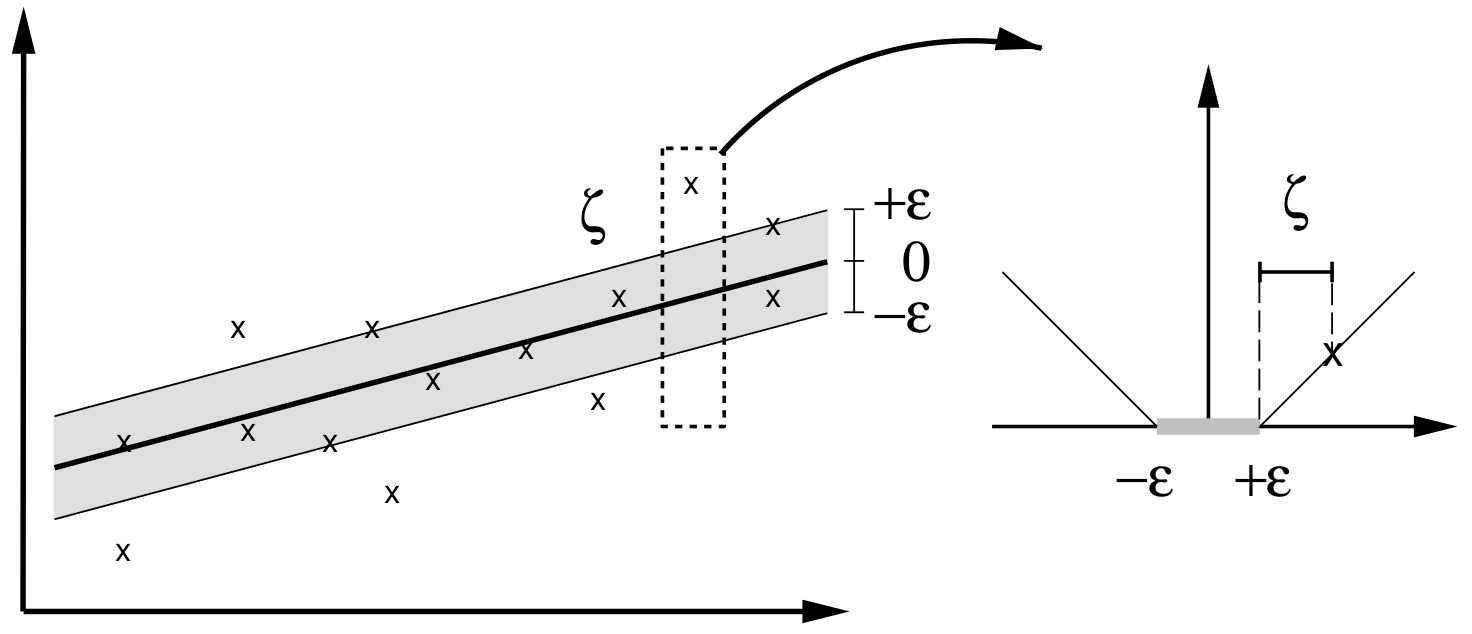
\includegraphics[width=8cm]{../img/epsilon_insensitive2.png}
\end{center}
\caption{Soft margin loss (from Sch\"olkopf and Smola, 2002)}
\label{fig:loss}
\end{figure}

The $\epsilon$-insensitive loss function defines the general case of the so-called $\epsilon$-SVR, whose corresponding optimization problem can be stated with the introduction of the slack variables $\xi_i$ and $\xi_i^*$

\begin{gather*}
\min\limits_{\beta,\beta_0} \frac{1}{2} \|w\|^2 + C \sum\limits_{i=1}^N \left(\xi_i + \xi_i^*\right)\\
\text{subject to }\left\{\begin{array}{rcl}
y_i-\langle w, x_i\rangle - b &\leq & \epsilon+\xi_i\\
\langle w, x_i\rangle +b -y_i &\leq & \epsilon +\xi_i^*\\
\xi_i, \xi_i^* & \geq & 0
\end{array}\right.
\end{gather*}

The $\xi_i$ slack variable can be interpreted as how much below the fitting plane $y_i$ really is, while $\xi_i^*$ represents how much above that plane $y_i$ stands. From there, the process is quite similar to the classification case. The objective function is quadratic and the constraints are linear. We introduce Lagrange multipliers $\alpha_i, \alpha_i^*, \eta_i, \eta_i^*$ and the (long) Lagrangian is:
\begin{multline*}
L = \frac{1}{2} \|w\|^2 + C \sum\limits_{i=1}^N \left(\xi_i + \xi_i^*\right)  - \sum\limits_{i=1}^N \alpha_i\left(\epsilon + \xi_i - y_i + \langle w, x_i\rangle + b\right)\\
-\sum\limits_{i=1}^N \alpha^*_i\left(\epsilon + \xi^*_i + y_i - \langle w, x_i\rangle - b\right) - \sum\limits_{i=1}^N \left(\eta_i\xi_i + \eta^*_i\xi^*_i\right)
\end{multline*}

The first order KKT condition is:
\begin{align*}
&\frac{\partial L}{\partial w} = w - \sum_{i=1}^N \left(\alpha_i-\alpha_i^*\right) x_i = 0\\
&\frac{\partial L}{\partial b} = \sum_{i=1}^N \left(\alpha_i^*-\alpha_i\right) = 0\\
&\frac{\partial L}{\partial \xi_i^{(*)}} = C - \alpha_i^{(*)} - \eta_i^{(*)}\\
&\forall i \in [1,N], \ \alpha_i\left(\epsilon + \xi_i - y_i + \langle w,x_i\rangle + b \right) = 0\\
&\forall i \in [1,N], \ \alpha^*_i\left(\epsilon + \xi^*_i - y_i + \langle w,x_i\rangle + b \right) = 0\\
&\eta_i \xi_i = 0\\
&\eta_i^* \xi_i^* = 0\\
&\alpha_i, \alpha_i^*, \eta_i, \eta_i^* \geq 0
\end{align*}

Just as in the classification case, using the three first equations above alow to transform the primal problem into the dual formulation. The dual function is:
\begin{equation*}
L_D = -\frac{1}{2}\sum\limits_{i=1}^N \sum\limits_{j=1}^N \left(\alpha_i - \alpha_i^*\right) \left(\alpha_j - \alpha_j^*\right) \langle x_i,x_j\rangle 
- \epsilon \sum\limits_{i=1}^N \left(\alpha_i + \alpha_i^*\right) + \sum\limits_{i=1}^N y_i \left(\alpha_i - \alpha_i^*\right)
\end{equation*}

And the dual optimization problem is:
\begin{gather*}
\max\limits_{\alpha} L_D\\
\text{subject to }\left\{\begin{array}{rcl}
\sum\limits_{i=1}^N \left(\alpha_i - \alpha^*_i\right) & = & 0\\
\alpha_i, \alpha_i^* & \in & [0,C]
\end{array}\right.
\end{gather*}

This problem can, again be solved through a variety of methods, the most commonly used being SMO (as in the classification case). The $b$ parameter is computed by using the $\alpha_i\left(\epsilon + \xi_i - y_i + \langle w,x_i\rangle + b \right)$ constraints for all $i$ such that $x_i$ is a support vector.

The first order condition allows a discussion on the Lagrange multipliers and the definition of the support vectors. First we use the $C - \alpha_i^{(*)} - \eta_i^{(*)}$ relationships to replace $\eta_i^{(*)}$ in the other equations to obtain:
\begin{align*}
&\alpha_i\left(\epsilon + \xi_i - y_i + \langle w,x_i\rangle + b \right) = 0\\
&\alpha^*_i\left(\epsilon + \xi^*_i - y_i + \langle w,x_i\rangle + b \right) = 0\\
&(C-\alpha_i) \xi_i = 0\\
&(C-\alpha_i^*) \xi_i^* = 0
\end{align*}

Then:
\begin{itemize}
\item if $\alpha_i^{(*)}=0$, then $\xi_i^{(*)}=0$: points inside the $\epsilon$-insensitivity ``tube'' don't participate in $w$
\item if $\alpha_i^{(*)}>0$ ($x_i$ is a support vector), then
\begin{itemize}
\item if $\xi^{(*)}_i = 0$, then $x_i$ is exactly on the border of the ``tube'', $\alpha_i^{(*)} \in [0,C]$
\item if $\xi^{(*)}_i > 0$, then $\alpha^{(*)}_i = C$: outliers are support vectors.
\end{itemize}
\end{itemize}
This interpretation is very similar to the case of classification with slack variables. Support vectors are example points that lie precisely on the insensitivity tube's border or outside this tube. All other points do not participate in defining $w$. Since $\alpha_i$ and $\alpha_i^*$ are zero for the majority of the training points, SVR retains the general property of sparsity: $w$ has a sparse extension in terms of $x_i$.

Given a new point $x$, the prediction step of an $\epsilon$-SVR consists in evaluating:
\begin{equation*}
f(x) = \sum\limits_{i=1}^N \left(\alpha_i-\alpha_i^*\right)\langle x_i,x \rangle + b
\end{equation*}

One issue that this paragraph does not adress is the question of automatically tuning the $\epsilon$ parameter along the optimization process. A refinement of the SVR problem, called $\nu$-SVR, extends $\epsilon$-SVR to the automatic tuning of the $\epsilon$ tube width.

The extension of the above development of SVR theory to the kernel-based case is straightforward.

\section*{Software}

\textbf{R.} In R, the \texttt{kernlab} and \texttt{e1071} libraries provide SVM computation, evaluation and plotting routines.

\textbf{C++ and others.} One of the most used SVM libraries is LIBSVM, with sources in C++ and Java, and interfaces to a wide variety of other languages.\\
\textbf{LIBSVM : a library for support vector machines.} Chih-Chung Chang and Chih-Jen Lin, \textit{ACM Transactions on Intelligent Systems and Technology}, \textbf{2}(3):27:1--27:27, 2011.\\
Software available at \verb#http://www.csie.ntu.edu.tw/~cjlin/libsvm#.

\textbf{Python.} In Python, the scikit-learn library provides classes for SVM use such as SVC or SVR.

\textbf{Weka.} Weka provides a nice graphical interface with SVM tools.

\end{document}
